\documentclass{standalone}
\usepackage{tikz}
\usetikzlibrary{arrows}
\begin{document}
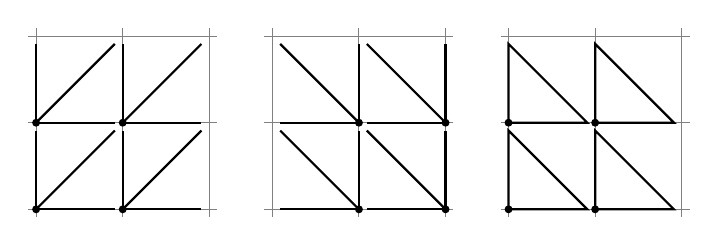
\begin{tikzpicture}[scale=.5]
\begin{scope}[shift={(0,0)}]
\foreach \i in {0,2.2,4.4}
	{\draw[gray] (-.2,\i) -- (4.6,\i);
	\draw[gray] (\i,-.2) -- (\i,4.6);}

\foreach \i in {0,2.2}
\foreach \j in {0,2.2}
	{\filldraw[thick] (0+\i,0+\j) circle (2pt) -- (2+\i,2+\j);
	\draw[thick] (0+\i,0+\j) -- (0+\i,2+\j);
	\draw[thick] (0+\i,0+\j) -- (2+\i,0+\j);}
\end{scope}

\begin{scope}[shift={(6,0)}]
\foreach \i in {0,2.2,4.4}
	{\draw[gray] (-.2,\i) -- (4.6,\i);
	\draw[gray] (\i,-.2) -- (\i,4.6);}

\foreach \i in {.2,2.4}
\foreach \j in {0,2.2}
	{\filldraw[thick] (2+\i,0+\j) circle (2pt) -- (0+\i,2+\j);
	\draw[thick] (2+\i,0+\j) -- (2+\i,2+\j);
	\draw[thick] (2+\i,0+\j) -- (0+\i,0+\j);}
\end{scope}

\begin{scope}[shift={(12,0)}]
\foreach \i in {0,2.2,4.4}
	{\draw[gray] (-.2,\i) -- (4.6,\i);
	\draw[gray] (\i,-.2) -- (\i,4.6);}

\foreach \i in {0,2.2}
\foreach \j in {0,2.2}
	{\filldraw[thick] (0+\i,0+\j) circle (2pt);
	\draw[thick] (0+\i,0+\j) -- (0+\i,2+\j) -- (2+\i,0+\j) -- cycle;}
\end{scope}
\end{tikzpicture}
\end{document}